\documentclass[11pt,a4paper]{article}


\setlength{\topmargin}{-55pt}%
\setlength{\oddsidemargin}{-20pt}%
\setlength{\textwidth}{490pt}%
\setlength{\textheight}{700pt}%
\setlength{\headsep}{20pt}%
\setlength{\headheight}{14pt}

\usepackage[utf8]{inputenc} % accents 8 bits dans le fichier
\usepackage[T1]{fontenc}      % accents codés dans la fonte
\usepackage[french]{babel}
\usepackage{amsmath,amssymb}
\usepackage{graphicx}
\usepackage{fancyhdr}
\usepackage{booktabs}
\usepackage{color, colortbl}
\usepackage{appendix}
\usepackage{pgfplots}
\usepackage[hidelinks]{hyperref}
\usepackage{siunitx}

\pgfplotsset{compat=1.3}

\addto\captionsfrench{% Replace "english" with the language you use
  \renewcommand{\contentsname}%
    {Table des matières}
}

\DecimalMathComma

\lhead{}      %en-tête
\chead{MPNA : Méthode des itérations simultanées}%
\rhead{}%
\lfoot{\tiny{Pierre GRANGER \& Matthias BEAUPERE}}
\cfoot{}%
\rfoot{\thepage}%
\renewcommand{\headrulewidth}{0.5pt}
\renewcommand{\footrulewidth}{0.5pt}
\pagestyle{fancy}

\newcommand{\HRule}{\rule{\linewidth}{0.5mm}}

\definecolor{green}{rgb}{0.2,0.8,0.2}

\begin{document}
\begin{center}

	{\LARGE\centering Projet de MPNA :\\ Méthode des itérations simultanées}\\[1cm]

	{ Matthias \bsc{Beaupère}, Pierre \bsc{Granger}}\\[0.5cm]
	{Rapport MPNA - CHPS - \today}
\end{center}

\tableofcontents

\section{Introduction}

\section{Problématique}

\section{Approche utilisée}

\section{Cas séquentiel}

	\subsection{Description de l'algorithme}
	\subsection{Etude de performances théorique}
	\subsection{Etude de performances pratique}
	\subsection{Ajout d'une méthode de déflation "locking"}
	\subsection{Conclusions}

\section{Cas parallèle}
	
	\subsection{Approche utilisée}
	\subsection{Etude de performances théorique}
	\subsection{Etude de performances pratique}
	\subsection{Conclusions}

\section{Conclusion générale}

% FIGURES A AJOUTER
\begin{figure}
	\centering
	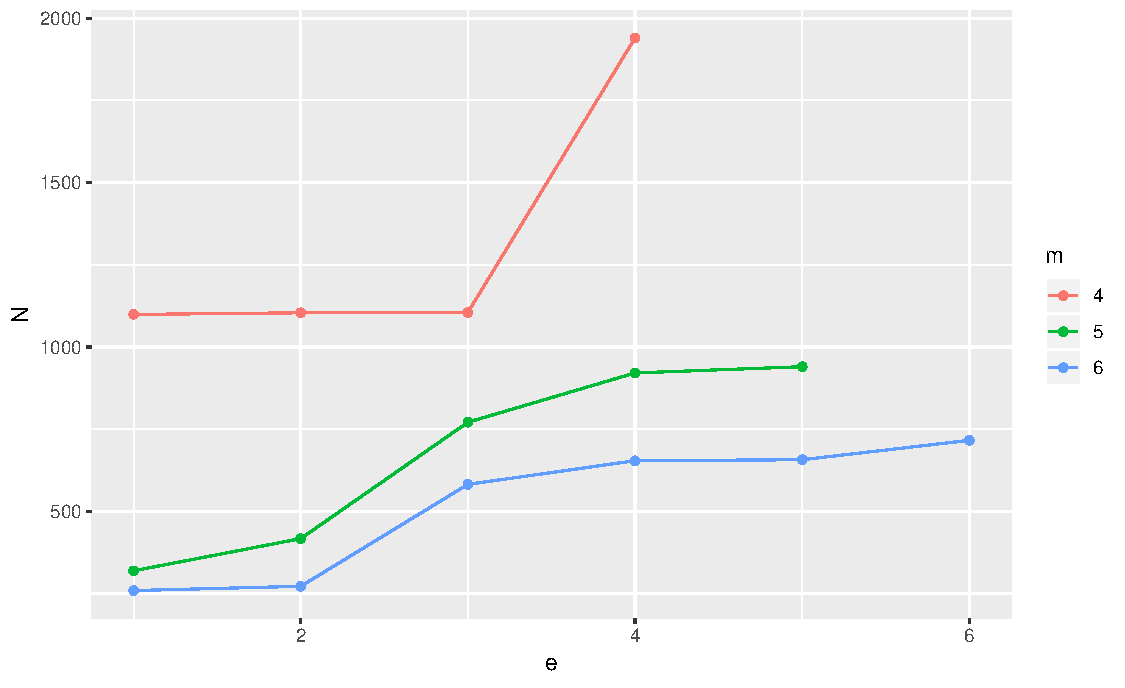
\includegraphics[width=0.8\linewidth, keepaspectratio]{plots/Nvse-m_p6.pdf}
	\caption{Nombre d'itérations $N$ nécessaires pour faire converger $e$ valeurs propres pour différentes tailles de sous-espace de Krylov $m$ et une précision $p=\SI{e-6}{}$ \label{fig:Nvse-m_p6}}
\end{figure}

\begin{figure}
	\centering
	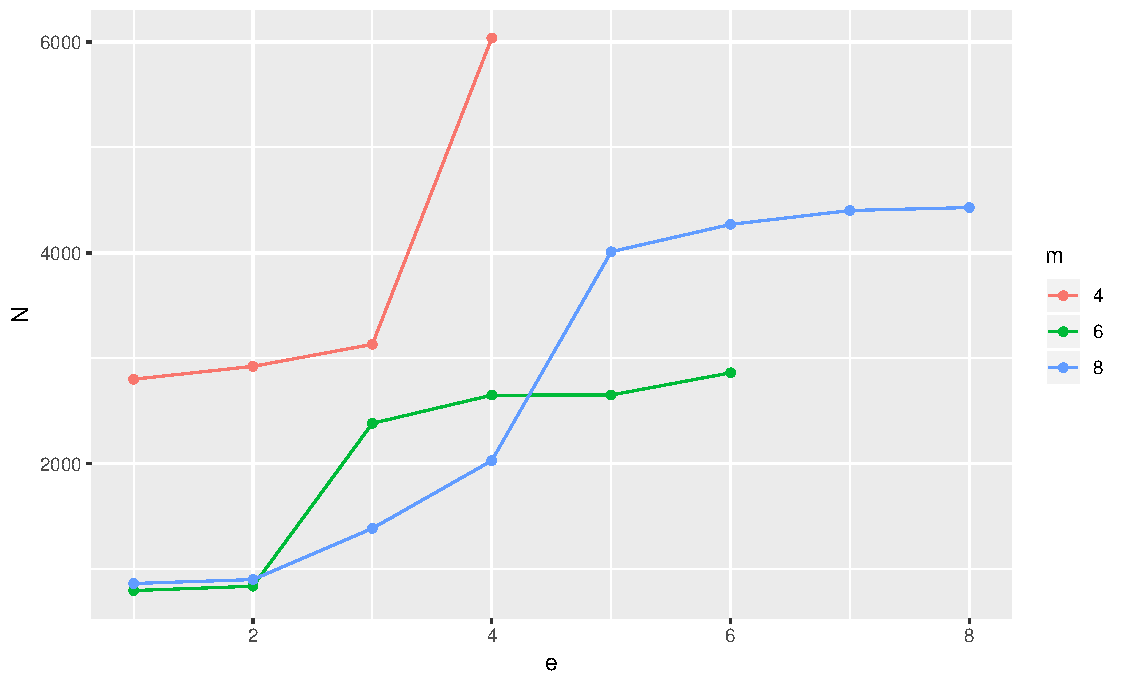
\includegraphics[width=0.8\linewidth, keepaspectratio]{plots/Nvse-m_p8.pdf}
	\caption{Nombre d'itérations $N$ nécessaires pour faire converger $e$ valeurs propres pour différentes tailles de sous-espace de Krylov $m$ et une précision $p=\SI{e-8}{}$ \label{fig:Nvse-m_p8}}
\end{figure}

\begin{figure}
	\centering
	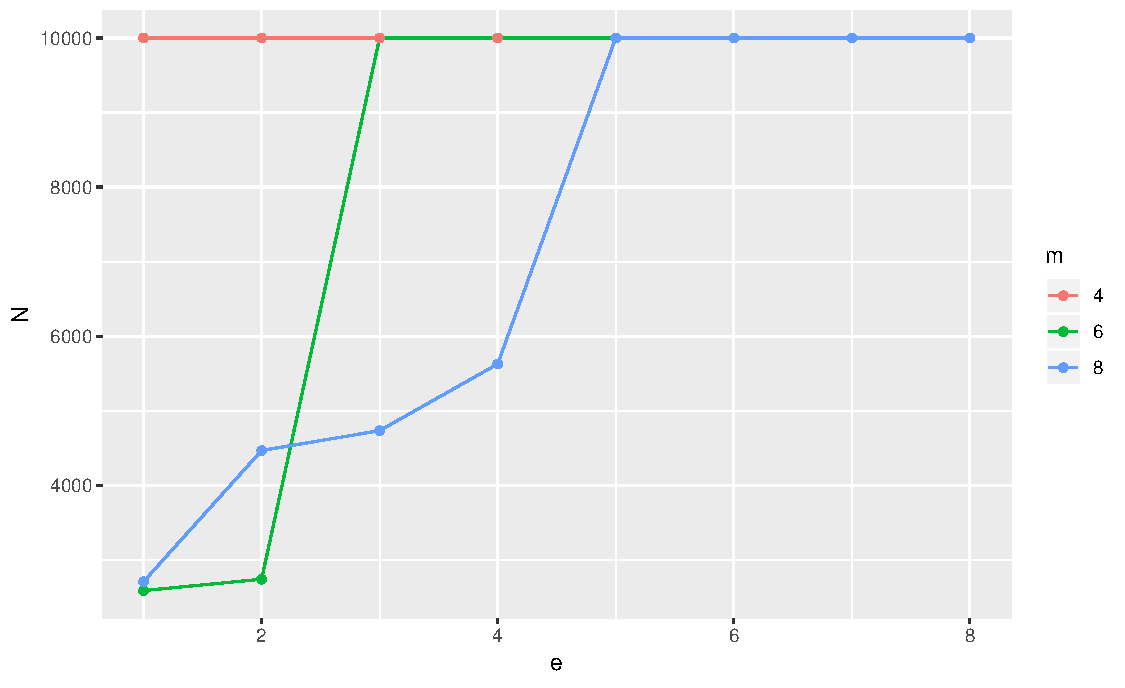
\includegraphics[width=0.8\linewidth, keepaspectratio]{plots/Nvse-m_p10.pdf}
	\caption{Nombre d'itérations $N$ nécessaires pour faire converger $e$ valeurs propres pour différentes tailles de sous-espace de Krylov $m$ et une précision $p=\SI{e-10}{}$ \label{fig:Nvse-m_p10}}
\end{figure}

\begin{figure}
	\centering
	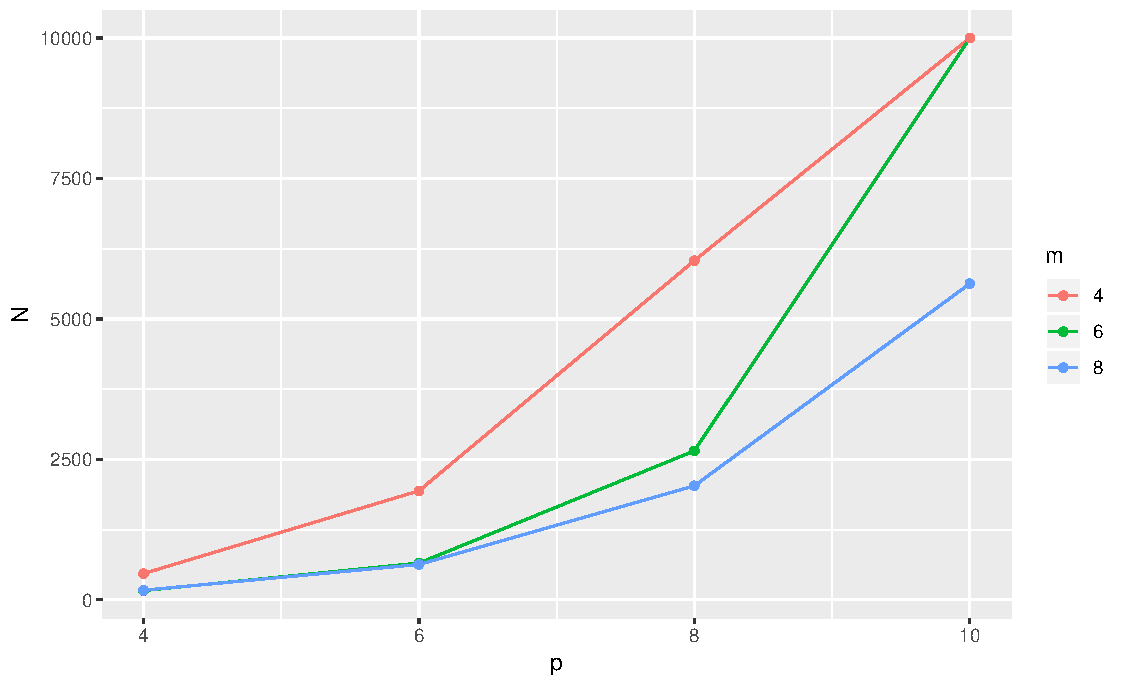
\includegraphics[width=0.8\linewidth, keepaspectratio]{plots/Nvsp-m_e4.pdf}
	\caption{Nombre d'itérations $N$ nécessaires pour faire converger $e = 4$ valeurs propres pour différentes tailles de sous-espace de Krylov $m$ et une précision $p$ \label{fig:Nvsp-m_e4}}
\end{figure}


% \bibliographystyle{unsrt}
% \bibliography{synopsis.bib}

%\input{appendix}

\end{document}
